\documentclass[13pt,a4paper]{article}
\usepackage{vntex}
\usepackage[left= 1in,right=0.79in,top= 1in,bottom=1in]{geometry}
\usepackage{a4wide,amssymb,epsfig,latexsym,multicol,array,hhline,fancyhdr}
\usepackage{mathptmx}
\usepackage{amsmath}
\usepackage{lastpage}
\usepackage[lined,boxed,commentsnumbered]{algorithm2e}
\usepackage{enumerate}
\usepackage{color}
\usepackage{graphicx}							% Standard graphics package
\usepackage{array}
\usepackage{tabularx, caption}
\usepackage{multirow}
\usepackage{multicol}
\usepackage{rotating}
\usepackage{graphics}
\usepackage{geometry}
\usepackage{setspace}
\usepackage{epsfig}
\usepackage{tikz}
\usetikzlibrary{arrows,snakes,backgrounds}
\usepackage{hyperref}
\hypersetup{urlcolor=blue,linkcolor=black,citecolor=black,colorlinks=true} 
\definecolor{mygreen}{RGB}{28,180,0} % color values Red, Green, Blue
\definecolor{mylilas}{RGB}{170,55,241}
\usepackage{listings}
\lstset{ 
	language=Matlab,                		% choose the language of the code
	%basicstyle=10pt,       				% the size of the fonts that are used for the code
	numbers=left,                  			% where to put the line-numbers
	numberstyle=\footnotesize,      		% the size of the fonts that are used for the line-numbers
	stepnumber=1,                   			% the step between two line-numbers. If it's 1 each line will be numbered
	numbersep=5pt,                  		% how far the line-numbers are from the code
	%	backgroundcolor=\color{white},  	% choose the background color. You must add \usepackage{color}
	showspaces=false,               		% show spaces adding particular underscores
	showstringspaces=false,         		% underline spaces within strings
	showtabs=false,                 			% show tabs within strings adding particular underscores
	%	frame=single,	                			% adds a frame around the code
	%	tabsize=2,                				% sets default tabsize to 2 spaces
	%	captionpos=b,                   			% sets the caption-position to bottom
	breaklines=true,                			% sets automatic line breaking
	breakatwhitespace=false,        		% sets if automatic breaks should only happen at whitespace
	escapeinside={\%*}{*)},          		% if you want to add a comment within your code
	emph=[1]{for,end,break,function},emphstyle=[1]\color{blue},
	stringstyle=\color{mylilas},
	commentstyle=\color{mygreen}
}
%\usepackage{fancyhdr}
\setlength{\headheight}{40pt}
\pagestyle{fancy}
\fancyhead{} % clear all header fields
\fancyhead[L]{
 \begin{tabular}{rl}
    \begin{picture}(25,15)(0,0)
    \put(0,-8){
\includegraphics[width=8mm, height=8mm]{images/hcmut.png}}
    %\put(0,-8){\epsfig{width=10mm,figure=hcmut.eps}}
   \end{picture}&
	%
\includegraphics[width=8mm, height=8mm]{hcmut.png} & %
	\begin{tabular}{l}
		\textbf{\bf \ttfamily Trường Đại Học Bách Khoa Tp.Hồ Chí Minh}\\
	\end{tabular} 	
 \end{tabular}
}
\fancyhead[R]{
	\begin{tabular}{l}
		\tiny \bf \\
		\tiny \bf 
	\end{tabular}  }
\fancyfoot{} % clear all footer fields
\fancyfoot[L]{\scriptsize \ttfamily Báo cáo lab 8 - Niên khóa 2019 - 2020}
\fancyfoot[R]{\scriptsize \ttfamily Trang {\thepage}/\pageref{LastPage}}
\renewcommand{\headrulewidth}{0.3pt}
\renewcommand{\footrulewidth}{0.3pt}


%%%
\setcounter{secnumdepth}{4}
\setcounter{tocdepth}{3}
\makeatletter
\newcounter {subsubsubsection}[subsubsection]
\renewcommand\thesubsubsubsection{\thesubsubsection .\@alph\c@subsubsubsection}
\newcommand\subsubsubsection{\@startsection{subsubsubsection}{4}{\z@}%
                                     {-3.25ex\@plus -1ex \@minus -.2ex}%
                                     {1.5ex \@plus .2ex}%
                                     {\normalfont\normalsize\bfseries}}
\newcommand*\l@subsubsubsection{\@dottedtocline{3}{10.0em}{4.1em}}
\newcommand*{\subsubsubsectionmark}[1]{}
\makeatother


\begin{document}

\begin{titlepage}
\begin{center}
ĐẠI HỌC QUỐC GIA THÀNH PHỐ HỒ CHÍ MINH \\
TRƯỜNG ĐẠI HỌC BÁCH KHOA \\
\end{center}

\vspace{1cm}

\begin{figure}[h!]
\begin{center}

\includegraphics[width=3cm]{images/hcmut.png}
\end{center}
\end{figure}

\vspace{1cm}


\large{KỸ NĂNG CHUYÊN NGHIỆP CHO KỸ SƯ}
\hline
\begin{center}
\textbf{{\huge THƯƠNG MẠI ĐIỆN TỬ}} \\
\textbf{{\huge TRONG HỘI NHẬP VÀ PHÁT TRIỂN}}
\end{center}
\\
\hline
\begin{center}
{\footnotesize TP. HỒ CHÍ MINH, THÁNG 6/2019}
\end{center}
\end{titlepage}
\newpage
\tableofcontents
\newpage
%%%%%%%%%%%%%%%%%%%%%%%%%%%%%%%%%
\fontsize{13pt}{1.2pt}\selectfont %chỉnh font và dãn dòng%
\section{Sơ lược về thương mại điện tử:}
Ngày nay thương mại điện tử đang ngày càng phát triển vượt bậc. Có bao giờ bạn thắc mắc "Thương mại điện tử là gì?". Bây giờ chúng ta sẽ cùng nhau quay về lịch sử để tìm hiểu về khái niệm và quá trình hình thành của Thương mại điện tử (TMĐT). Đầu tiên, TMĐT là việc tiến hành một phần hay toàn bộ hoạt động kinh doanh bằng các phương tiện điện tử. Một cách dễ hiểu hơn thì thương mại điện tử chính là việc mua bán sản phẩm hay dịch vụ thông qua internet và các phương tiện điện tử khác. Các giao dịch này bao gồm tất cả các hoạt động như: giao dịch, mua bán, thanh toán, đặt hàng, quảng cáo và giao hàng… \\ \\
\begin{center}
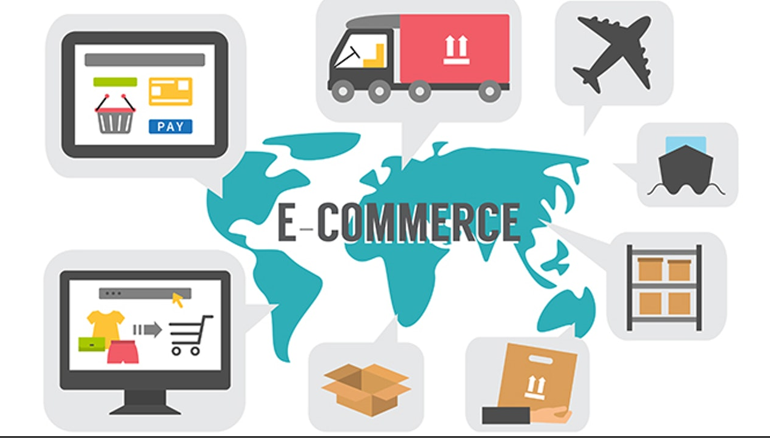
\includegraphics[scale=0.5]{images/e-com.png}\\
\fontsize{10pt}{1.2pt}\selectfont
    Source: https://devteam.mobi/e-commerce-la-gi-tim-hieu-chi-tiet-ve-e-commerce/
\\
\end{center}
TMĐT xuất hiện vào những năm 1980, phần lớn là dân chủ hóa vào cuối những năm 1990 với sự xuất hiện của thanh toán trực tuyến và sự dân chủ hóa truy cập Internet trong từng hộ gia đình.
IBM và Microsoft là những người tiên phong đầu tiên sử dụng khái niệm “thương mại điện tử” này, các sản phẩm được chào bán chủ yếu là hàng máy tính.
\\\begin{center}

\includegraphics[scale=0.5]{images/IBM.png}\\
\end{center}
\section{Cách thức hoạt động:} 
\section{Xu hướng phát triển:}
    \subsection{Giới thiệu sản phẩm bằng video livestream:}\\
    Điều duy nhất mà mua sắm online không thể canh tranh với mua tại cửa hàng là sự trải nghiệm trực tiếp sản phẩm. Tuy nhiên ngày nay người dùng không cần đến cửa hàng vẫn có thể trải nghiệm sản phẩm tại nhà thông qua các video live stream trên facebook, youtube, instagram,... và các phương tiện truyền thông có tính năng livestream khác,...\\
    \\\begin{center}
    
\includegraphics[scale=0.6]{images/f&u.png} \\
    \fontsize{10pt}{1.2pt}\selectfont
    Source: https://tintuc.shopdunk.com/livestream-khi-choi-game-len-facebook-va-youtube.html
    \end{center}
    \subsection{Phát triển quảng cáo bằng mạng xã hội và youtube:}
    Trong XH hiện đại như bây giờ thì nhu cầu sử dụng mạng XH ngày càng tăng cao. Các dịch vụ quảng cáo qua mạng XH cũng từ đó mà không ngừng phát triển.
    Bây giờ các bạn có thể dễ dàng bắt gặp những quảng cáo như: “Nếu tình yêu của bạn không thuận thì không phải do bạn không tốt chỉ là do bạn chưa gặp đúng người thôi – Spoon mạng XH âm thanh. Đôi lúc những quảng cáo ngày sẽ tạo cho bạn một sự khó chịu nhất định
     \\\begin{center}
    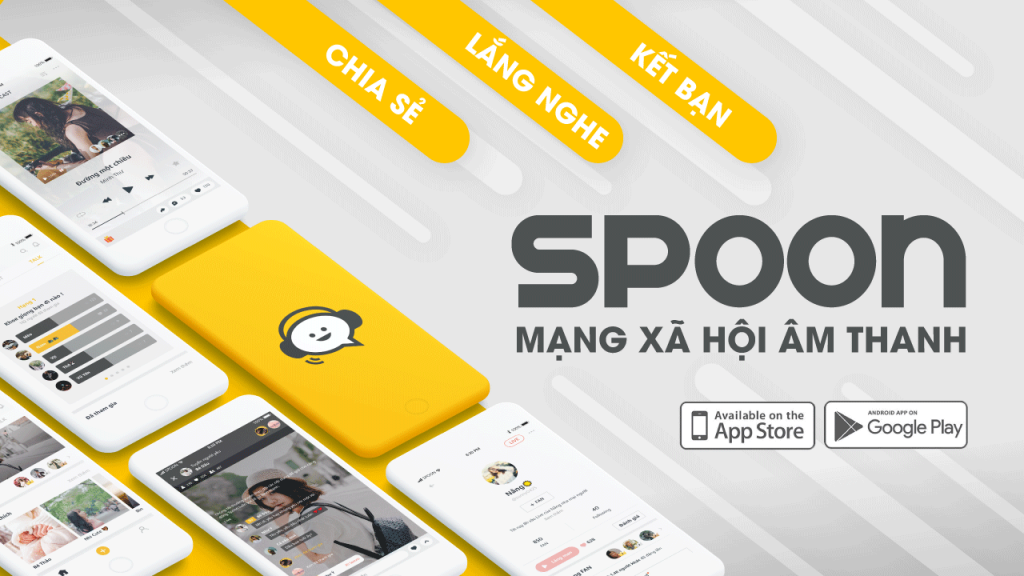
\includegraphics[scale=0.25]{images/spoon.png} \\
    \fontsize{10pt}{1.2pt}\selectfont
    Source: https://spooncast.vn/mang-xa-hoi-am-thanh-spoon-radio/
    \end{center}
    \\
    Và gần đây chúng ta có thể dễ dàng bắt gặp sự xuất hiện của Tiki tràn ngập các MV ca nhạc của những nghệ sĩ đình đám như: Đức Phúc, Hiền Hồ, Chipu,..
    \\\begin{center}
    
\includegraphics[scale=0.8]{images/tiki.png} \\
    \fontsize{10pt}{1.2pt}\selectfont
    Source: https://wikimarketing.vn/tiki-di-cung-sao-viet.html/
    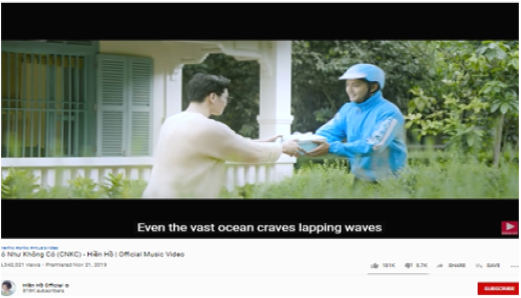
\includegraphics[scale=0.7]{images/conhungkhongco.png} \\
    \fontsize{10pt}{1.2pt}\selectfont
    Source: https://www.youtube.com/watch?v=dsri8IJI6rY
    \end{center}
    \subsection{Nỗ lực về dịch phụ giao hàng:}\\
    Giao hàng là chìa khóa dẫn đến sự hài lòng của khách hàng. Một khảo sát của iPrice về mua sắm trong khu vực Đông Nam Á cho thấy mỗi khi nào thời gian giao hàng kéo dài, tỷ lệ khách hàng hài lòng với xếp hạng 4-5 sao sẽ giảm từ 10 - 15 phần trăm . Rất nhiều khách hàng ưu tiên việc nhận sản phẩm sớm và sẵn sàng trả nhiều tiền hơn cho việc chuyển phát nhanh hoặc trong ngày.\\
    Để đáp ứng nhu cầu này từ khách hàng, các công ty nên hợp tác với các đơn vị hậu cần thứ ba để cung cấp nhiều phương thức vận chuyển khác nhau nhằm giúp khách hàng dễ dàng lựa chọn dịch vụ vận chuyển
    \begin{center}
    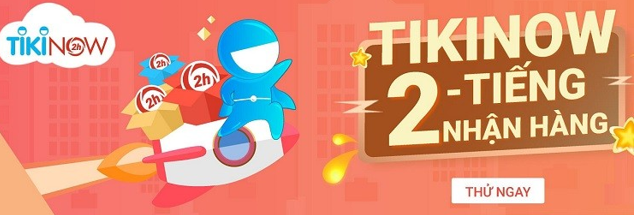
\includegraphics[scale=0.6]{images/giaohang.png} \\
    \fontsize{10pt}{1.2pt}\selectfont
    Source: https://www.foody.vn/bai-viet/trai-nghiem-dich-vu-nowship-giao-hang-tuc-thoi-uu-dai-cuc-hap-dan-18024
    \end{center}
    \subsection{Thanh toán trực tuyến:}\\
    Ngày nay, thay vì phải đến trực tiếp cửa hàng để chọn lựa, mua hàng và thanh toán bằng tiền mặt hay quẹt thẻ ATM thì khách hàng thời đại 4.0 chỉ cần ở nhà cầm một chiếc điện thoại đặt hàng và thanh toán bằng các dịch vụ thanh toán trực tiếp.
    Hiện nay, ở Việt Nam ví điện tử đang phát triển rất mạnh mẽ, điển hình là Momo, AirPay, Moca, Zalo Pay,...
    \begin{center}
    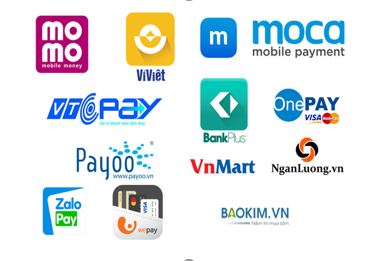
\includegraphics[scale=1]{images/vi.png} \\
    \fontsize{10pt}{1.2pt}\selectfont
    Source: https://www.foody.vn/bai-viet/trai-nghiem-dich-vu-nowship-giao-hang-tuc-thoi-uu-dai-cuc-hap-dan-18024
    \end{center}
    Theo báo cáo của Google, thanh toán trực tuyến đã đạt đến điểm chuyển ngoặt với tỷ lệ sử dụng ngày càng tăng trong khu vực. Với tổng giá trị giao dịch (Gross Transaction Value - GTV) 600 tỉ đô la vào năm 2019, mảng thanh toán trực tuyến được dự đoán sẽ vượt mức 1 nghìn tỷ đô la vào năm 2025, chiếm gần một nửa tổng giá trị thanh toán của người tiêu dùng trong khu vực. \\
    Mặc dù phương thức thanh toán phổ biến nhất hiện tại là trả tiền mặt khi nhận hàng (Cash on Delivery - CoD),nhưng thanh toán trực tuyến cũng đang dần khẳng định vị trí của mình trong thế giới công nghệ hoá. \\
    Ngoài ra, trên các dịch vụ thanh toán trực tiếp còn cung cấp cho người dùng rất nhiều mã giảm giá như sale off 30 phần trăm, 50 phần trăm, mã freeship,..được cập nhật liên tục hằng ngày để người dùng thoải mái lựa chọ.
    \begin{center}
    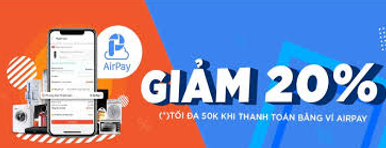
\includegraphics[scale=0.9]{images/giam.png} \\
    \fontsize{10pt}{1.2pt}\selectfont
    Source: https://magiamgiashopee.vn/huong-dan-lien-ket-airpay-voi-shopee/
    \end{center}
    \subsection{Dịch vụ đăng kí:}
    Các dịch vụ đăng kí cũng là một dạng thương mại điển tử và đang phát triển với tốc độ vượt bậc ở Việt Nam và trên thế giới. Trong thời gian dịch Covid 19 diễn ra thì chắc hẳn mọi người sẽ có nhiều thời gian rảnh rỗi, và nghe nhạc và xem phim để giải trí cũng là sự lựa chọn của rất nhiều người dùng. Và vì vậy đó là lí do mà các dịch vụ đăng kí đạt đến sự phát triển mạnh mẽ. Điển hình là kênh xem video và phim với lượt đăng kí khủng: Netflix hay là dịch vụ nghe nhạc Spotify.
    \begin{center}
    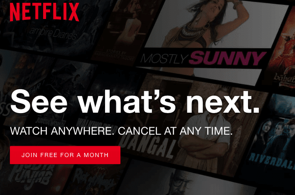
\includegraphics[scale=0.85]{images/net.png} 
    \fontsize{10pt}{1.2pt}\selectfont \quad 
\includegraphics[scale=1.1]{images/spot.png} \\
    \fontsize{10pt}{1.2pt}\selectfont
    \end{center}
\section{Thực trạng:}\\ 
\section{Lợi ích và thách thức:}\\
    \subsection{Ảnh hưởng bởi sự phát triển thương mại điện tử nước ngoài}\\
    Bên cạnh những lợi ích mà thương mại điện tử đem lại cho người dùng thì nó vẫn còn tồn tại những thách thức và rào cản khiến TMĐT Việt Nam không thể cạnh tranh với các nước khác trên trường quốc tế.\\ 
    Hiện nay, người tiêu dùng Việt Nam, đặc biệt là thế hệ người tiêu dùng trẻ hiện khá ưa chuộng mua hàng qua các website thương mại điện tử của nước ngoài như Amazon, eBay… do hàng hóa của nước ngoài phong phú, đa dạng và phù hợp với đại đa số người tiêu dùng, đặc biệt là giới trẻ thành thị, trong khi chi phí phải trả cho việc mua hàng trực tuyến từ nước ngoài thường thấp hơn trong nước…
    \subsection{Môi trường cạnh tranh khốc liệt:}\\
     Môi trường cạnh tranh khốc liệt không dành cho các DN có năng lực tài chính, công nghệ, quản trị… yếu kém,… đòi hỏi phải cạnh tranh chạy đua giữa những doanh nghiệp trong và ngoài nước. Những doanh nghiệp có trình độ phát triển yếu kém hơn sẽ nhanh chóng bị đào thải. 
     \begin{center}
    
\includegraphics[scale=0.8]{images/thach.png} \\
    \fontsize{10pt}{1.2pt}\selectfont
    \end{center}
    \subsection{Cơ sở hạ tầng chưa đáp ứng đủ cho sự phát triển:}\\
    Cơ sở hạ tầng công nghệ chưa tốt không chỉ khiến cho thương mại điện tử của Việt Nam khó cạnh tranh với các quốc gia phát triển khác có thể đối mặt với các sự cố không mong muốn hoặc thách thức về an ninh mạng. Thống kê của Lazada tại Diễn đàn Toàn cảnh Thương mại điện tử 2017, trong sự kiện cáp quang AAG bị đứt vào 2,3 tuần năm 2016, Lazada đã mất tới 30 phần trăm doanh thu trung bình trong một ngày.
    \subsection{Vấn đề bảo mật:}\\
    Bên cạnh đó, vấn đề an ninh, an toàn, bảo mật thông tin… trên các giao dịch điện tử vẫn chưa thể khiến người tiêu dùng an tâm.
    \begin{center}
    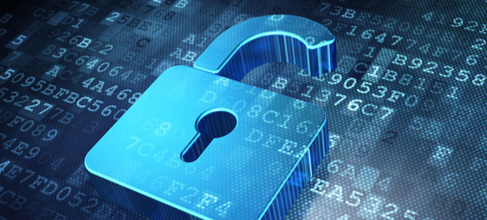
\includegraphics[scale=0.8]{images/khoa.png} \\
    \fontsize{10pt}{1.2pt}\selectfont
    \end{center}
    
\section{Tác hại, hậu quả và biện pháp khắc phục:}



	
	


%%%%%%%%%%%%%%%%%%%%%%%%%%%%%%%%%
\newpage


\end{document}





\end{document}

